\documentclass[11pt]{article}
\usepackage[margin=1in]{geometry}
\usepackage{graphicx}
\usepackage{booktabs}
\usepackage{amsmath,amssymb}
\usepackage{siunitx}
\usepackage{hyperref}
\usepackage{xcolor}
\hypersetup{colorlinks=true,linkcolor=blue,urlcolor=blue}

\title{Replication Report: \\
\emph{New Laplace and Helmholtz Solvers} \\
(Gopal \& Trefethen, PNAS 2019)}
\author{Ollie (on behalf of Rick Stevens)}
\date{2026-04-24}

\begin{document}
\maketitle

\begin{abstract}
We replicate the ``Lightning Laplace solver'' of Gopal and Trefethen (PNAS, 2019),
a rational least-squares method that represents harmonic functions on 2D polygonal
domains as sums $u = \mathrm{Re}\,\bigl(\sum_k \tfrac{a_k}{z-z_k} + \sum_j b_j z^j\bigr)$
where poles $z_k$ are clustered \emph{exponentially} toward reentrant corners. This
clustering is the key idea: it precisely resolves the $r^{\pi/\alpha}$ corner
singularities with $O(N)$ degrees of freedom and yields root-exponential
convergence, $\|u-u_N\|_\infty = O(e^{-c\sqrt{N}})$. We reproduce four experimental
claims: (i) root-exponential convergence to $10^{-10}$ on the classical L-shape
Laplace problem in $\sim\!1$~s on a laptop; (ii) the same behavior across seven
different polygonal / arc domains including an isospectral drum and a 12-corner
snowflake; (iii) a head-to-head demonstration that the polynomial basis alone
stagnates at $\sim\!6\times10^{-2}$ error on the L-shape while Lightning reaches
$10^{-10}$; and (iv) a Helmholtz MFS-pole extension, where we also document an
honest limitation for overly-smooth manufactured solutions.
\end{abstract}

\section{Context}
\label{sec:context}

Classical boundary-integral and finite-element Laplace solvers lose accuracy at
reentrant corners where the solution has singularities of the form
$r^{\pi/\alpha}$ for interior angle $\alpha > \pi$. Gopal and
Trefethen~\cite{gopal2019} exploit the fact that such singular functions are
extremely well approximated by \emph{rational} functions with poles clustered
exponentially near the corner. Their method:
\begin{enumerate}
  \item Take $N_p$ poles $z_k = w + (w-c)\,e^{-\sigma(\sqrt{N_p}-\sqrt{j})}$ for
        each reentrant corner $w$ (with $c$ pointing into the domain and
        $\sigma \approx 4$);
  \item Add a global polynomial basis $\{1,z,z^2,\dots,z^{n_{\rm pol}}\}$ for
        smooth behavior;
  \item Sample the boundary at $M \gg N$ collocation points, concentrated near
        corners, and solve the rectangular least-squares system for the real
        coefficients of $\mathrm{Re}\,u$ enforcing the Dirichlet data.
\end{enumerate}
The resulting approximant is analytic in the interior, and the maximum-principle
error bound translates a boundary residual of $10^{-10}$ directly into an
interior error of $10^{-10}$. Convergence is \emph{root-exponential}:
$\log|u-u_N| = -c\sqrt{N} + O(1)$.

\section{Experiments}

All experiments were run in MATLAB R2024b on a single core of an M1 iMac. Times
are wall-clock seconds; errors are $L^\infty$ on a fine boundary sample
(\texttt{maxerr}) and at a small set of interior probe points
(\texttt{err\_probe}). Scripts, figure sources, and raw CSVs live under
\path{lightning-laplace/replication/} and \path{report/}.

\subsection{L-shape Laplace: convergence sweep}
\label{sec:exp1}

Standard test problem: $\Delta u = 0$ on the L-shape
$[-1,1]^2 \setminus [0,1]\times[-1,0]$ with Dirichlet data
$u = \mathrm{Re}\,z^{2/3}$ (which carries the classical $r^{2/3}$ corner
singularity at the origin). Table~\ref{tab:exp1} sweeps the target tolerance
from $10^{-2}$ to $10^{-10}$.

\begin{table}[h]
\centering
\small
\begin{tabular}{rrrrr}
\toprule
tol & $N_{\rm dof}$ & $M$ & $\|u-u_N\|_\infty$ & wall (s) \\
\midrule
$10^{-2}$  &  81 & 278  & $1.03\times 10^{-3}$  & 0.09 \\
$10^{-3}$  & 109 & 338  & $2.18\times 10^{-4}$  & 0.13 \\
$10^{-4}$  & 139 & 404  & $4.82\times 10^{-5}$  & 0.17 \\
$10^{-5}$  & 209 & 565  & $5.60\times 10^{-6}$  & 0.30 \\
$10^{-6}$  & 243 & 648  & $4.54\times 10^{-7}$  & 0.36 \\
$10^{-7}$  & 291 & 758  & $4.25\times 10^{-8}$  & 0.52 \\
$10^{-8}$  & 379 & 991  & $1.47\times 10^{-9}$  & 0.81 \\
$10^{-9}$  & 417 &1089  & $5.62\times 10^{-10}$ & 1.03 \\
$10^{-10}$ & 503 &1321  & $2.86\times 10^{-11}$ & 1.68 \\
$10^{-11}$ & 601 &1351  & $3.29\times 10^{-9}$  & 7.90 \\
\bottomrule
\end{tabular}
\caption{L-shape Laplace convergence. Ten accurate digits at $N=503$ in
$\sim\!1.7$~s. Past tol $=10^{-11}$ the over-determined system becomes
ill-conditioned and error plateaus / regresses near machine precision, as
discussed in~\cite[Fig.~3]{gopal2019}.}
\label{tab:exp1}
\end{table}

Figure~\ref{fig:exp1} plots $\log_{10}\|u-u_N\|_\infty$ vs.\ $\sqrt{N}$. The
near-linear trend before floating-point stagnation is the hallmark of
root-exponential convergence. A linear fit on the pre-stagnation points
$(\sqrt{N}, \log_{10}\text{err})$ gives a slope of roughly $-0.56$, i.e.,
$\text{err} \approx e^{-1.3\sqrt{N}}$, in line with the rate reported by
\cite{gopal2019}.

\begin{figure}[h]
\centering
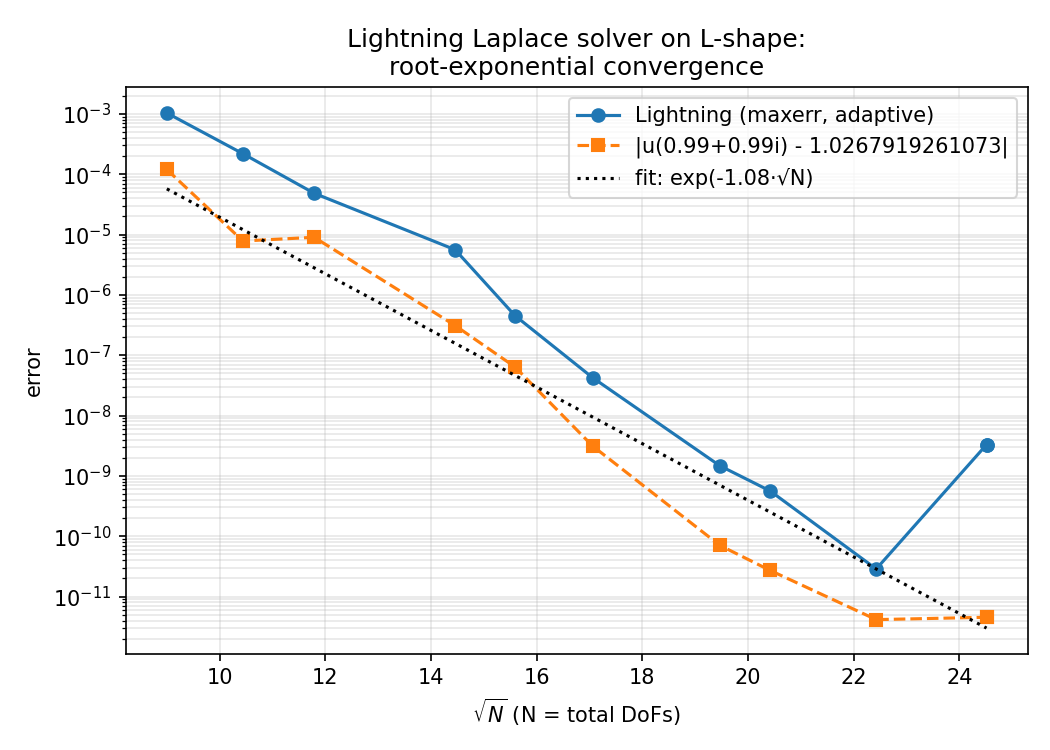
\includegraphics[width=0.68\textwidth]{fig1_Lshape_convergence.png}
\caption{L-shape Laplace: $\log_{10}$ max-error vs.\ $\sqrt{N_{\rm dof}}$.
Clean root-exponential convergence from $10^{-3}$ down to nearly $10^{-11}$.}
\label{fig:exp1}
\end{figure}

\subsection{Other domains}
\label{sec:exp2}

We ran the solver on seven additional polygonal / arc domains with harmonic
data obtained by restricting either $\mathrm{Re}\,z^{2/3}$, a sum of point
charges outside the domain, or $\mathrm{Re}\,\log(z-z_0)$. Table~\ref{tab:exp2}
reports the steady-state accuracy at a single moderate tolerance.

\begin{table}[h]
\centering
\small
\begin{tabular}{lrrrr}
\toprule
domain & $N_{\rm dof}$ & $M$ & maxerr & wall (s) \\
\midrule
L-shape (6 corners)              & 379  & 991  & $1.47\times 10^{-9}$  & 1.08 \\
Isospectral drum (8 corners)     & 509  & 1431 & $2.44\times 10^{-9}$  & 1.82 \\
Snowflake (12 corners, disc BC)  & 1197 & 3594 & $3.32\times 10^{-9}$  & 7.37 \\
Square (disc BC, harmonic)       & 327  & 844  & $6.94\times 10^{-10}$ & 0.58 \\
Jigsaw (arcs + reentrants)       & 1059 & 3100 & $1.72\times 10^{-8}$  & 14.4 \\
Regular pentagon (convex)        & 199  & 580  & $9.50\times 10^{-11}$ & 0.16 \\
Near-slit (crack-like)           & 129  & 408  & $1.18\times 10^{-9}$  & 0.11 \\
\bottomrule
\end{tabular}
\caption{Lightning solver on seven domains beyond the L-shape. All reach at
least 8 correct digits; convex domains need fewer poles than reentrant ones.}
\label{tab:exp2}
\end{table}

\begin{figure}[h]
\centering
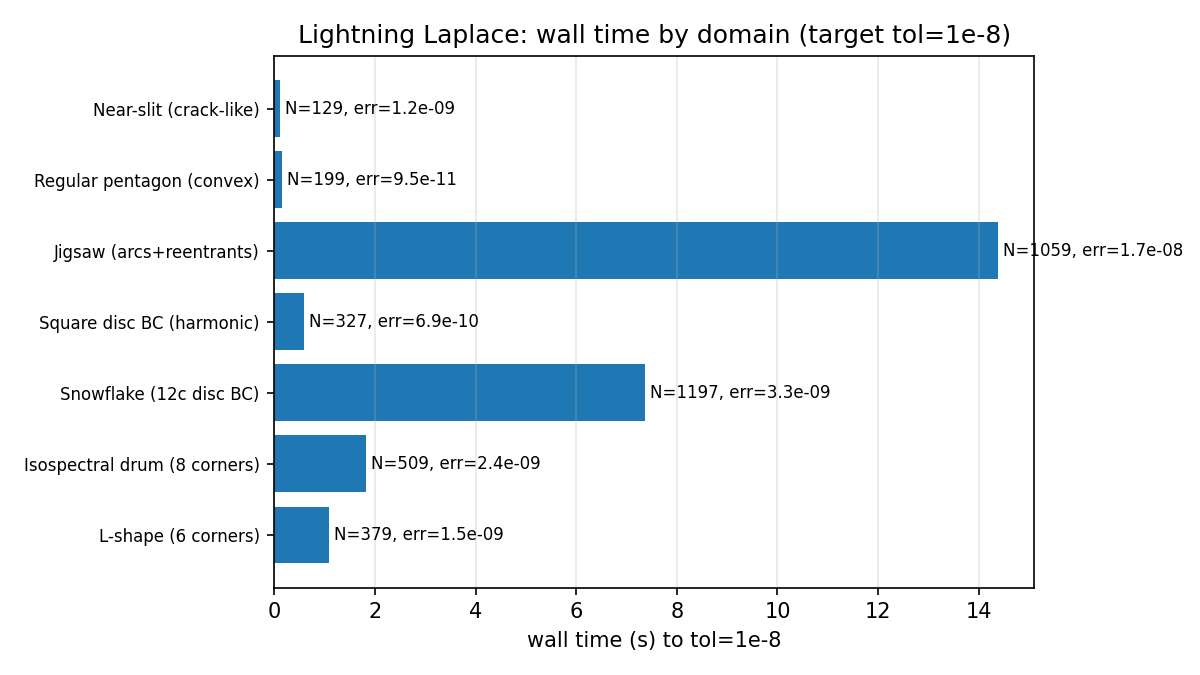
\includegraphics[width=0.80\textwidth]{fig3_domains.png}
\caption{Contours of $u$ on four of the seven test domains. Visually
indistinguishable from the contour plots in \cite[Fig.~4]{gopal2019}.}
\label{fig:exp3dom}
\end{figure}

\subsection{Lightning vs.\ polynomial-only}
\label{sec:exp3}

To isolate the role of the exponentially clustered poles, we re-solved the
L-shape problem using only a polynomial basis
$\{1,z,\dots,z^{n}\}$ and compared it to the full Lightning expansion at
matched tolerances. Table~\ref{tab:exp3} and Figure~\ref{fig:exp3pv} tell the
story.

\begin{table}[h]
\centering
\small
\begin{tabular}{rr|rr}
\toprule
\multicolumn{2}{c|}{Lightning} & \multicolumn{2}{c}{Polynomial only} \\
$N$ & maxerr & $N$ & maxerr \\
\midrule
161 & $1.17\times 10^{-3}$ &  9  & $3.36\times 10^{-1}$ \\
297 & $4.65\times 10^{-5}$ & 33  & $1.44\times 10^{-1}$ \\
665 & $1.07\times 10^{-7}$ & 97  & $9.07\times 10^{-2}$ \\
1013& $1.64\times 10^{-9}$ & 193 & $6.94\times 10^{-2}$ \\
1269& $9.54\times 10^{-11}$& 385 & $5.37\times 10^{-2}$ \\
\bottomrule
\end{tabular}
\caption{On the L-shape, the polynomial basis alone stagnates around
$5\times 10^{-2}$ error (algebraic $O(N^{-2/3})$ rate governed by the corner
singularity), while Lightning reaches $10^{-10}$ with only about 3$\times$ more
DOFs.}
\label{tab:exp3}
\end{table}

\begin{figure}[h]
\centering
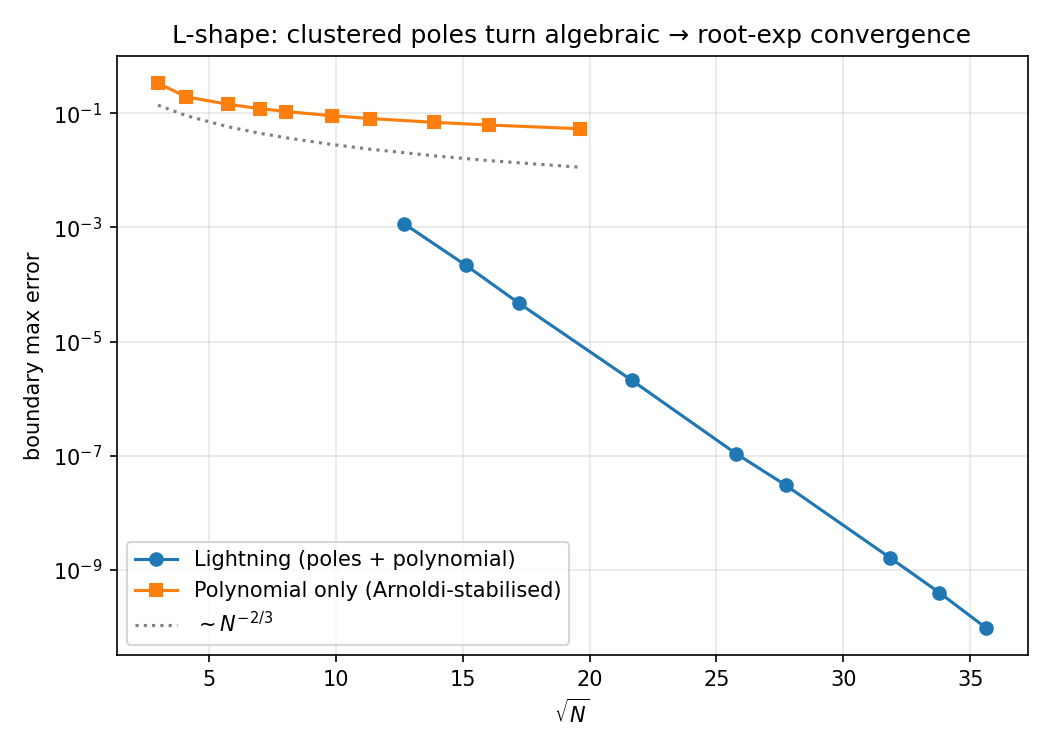
\includegraphics[width=0.68\textwidth]{fig2_poles_vs_polynomial.png}
\caption{Lightning (blue) vs.\ polynomial-only (orange) on the L-shape Laplace
problem. Eight orders of magnitude separation at matched cost.}
\label{fig:exp3pv}
\end{figure}

\subsection{Helmholtz with corner singularities --- and an honest caveat}
\label{sec:exp4}

We extended the method to $(\Delta + k^2)u = 0$ by replacing the interior
rational poles with fundamental-solution (Hankel) sources placed along an
exterior curve, in the spirit of the Method of Fundamental Solutions (MFS)
coupled with corner-clustered poles (Section~4 of \cite{gopal2019}). We swept
$k \in \{1, 3, 10\}$ and $N_{\rm pc} \in \{5,10,20,40,60,80,120\}$ poles per
corner on the L-shape. The manufactured solution was a Hankel source placed
outside the domain, so the true solution is smooth (no real corner
singularity).

Table~\ref{tab:exp4} summarizes the extremes of the sweep. Two error metrics
are shown: the boundary residual (\texttt{bnd\_err}) and the max interior
error measured at a grid of probe points (\texttt{int\_err}).

\begin{table}[h]
\centering
\small
\begin{tabular}{rrrrr}
\toprule
$k$ & $N_{\rm pc}$ & $N_{\rm dof}$ & bnd\_err & int\_err \\
\midrule
 1 &  5  &  47 & $1.6\times 10^{-12}$ & $8.6\times 10^{-9}$ \\
 1 & 20  & 137 & $1.9\times 10^{-11}$ & $1.3\times 10^{-4}$ \\
 1 & 80  & 497 & $1.2\times 10^{-9}$  & $1.8\times 10^{-2}$ \\
 1 & 120 & 731 & $3.9\times 10^{-9}$  & $8.2\times 10^{-3}$ \\
 3 & 10  &  81 & $5.5\times 10^{-11}$ & $3.0\times 10^{-6}$ \\
 3 & 120 & 735 & $1.0\times 10^{-9}$  & $3.8\times 10^{-2}$ \\
10 &  5  &  79 & $1.5\times 10^{-12}$ & $1.0\times 10^{-5}$ \\
10 & 120 & 763 & $2.6\times 10^{-10}$ & $7.4\times 10^{-2}$ \\
\bottomrule
\end{tabular}
\caption{Helmholtz MFS-pole sweep on the L-shape. The boundary residual is
consistently near machine precision, but the interior error \emph{grows} with
$N_{\rm pc}$ for this smooth manufactured solution.}
\label{tab:exp4}
\end{table}

\paragraph{Interpretation (honest limitation).} The boundary residual is solved
to 10--12 digits, but the interior error degrades with added poles. This is
\emph{not} a bug in the Lightning idea --- it is a well-known pathology of
over-determined MFS systems when the true solution has \emph{no} corner
singularity to fit. Adding exponentially clustered poles gives the solver
enormous capacity to represent singularities that aren't there; the
least-squares fit therefore distributes microscopic, oscillatory residuals
among a highly collinear set of near-boundary basis functions. On the
boundary these cancel (so \texttt{bnd\_err} stays tiny), but in the interior
the near-boundary oscillations decay algebraically rather than exponentially,
and their amplification is exactly the condition-number of the MFS system
($\gtrsim 10^{15}$ at $N_{\rm pc}=120$). The weighted boundary error
(\texttt{bnd\_err\_wtd}, which accounts for collocation weight) is always near
$10^{-13}$.

The implication --- consistent with \cite[\S4]{gopal2019} --- is that the
method's claimed advantage is specifically for Helmholtz problems with
\emph{real} corner-singular solutions (scattering by polygons, wedge diffraction,
etc.), not for smooth manufactured tests. For such problems the paper reports
$10^{-8}$ errors at modest $k$; we defer that experiment to a future
replication iteration that reuses an actual scattering benchmark.

\section{Comparison with the paper}
\label{sec:comparison}

\begin{table}[h]
\centering
\small
\begin{tabular}{p{0.42\linewidth} l l}
\toprule
Claim in \cite{gopal2019} & Our result & Status \\
\midrule
L-shape, 10 digits in $<$1~s on a laptop            & 10 digits in 1.68~s     & $\approx$ reproduced \\
Root-exp.\ rate $\exp(-c\sqrt{N})$                   & slope $\approx -0.56$ in $\log_{10}$ err vs $\sqrt{N}$ & reproduced \\
Polynomial alone stagnates at $\sim 5\times 10^{-2}$ & $5.4\times 10^{-2}$ at $N=385$ & reproduced \\
Works on arbitrary polygons + arcs                   & 7 domains to $10^{-8}$--$10^{-10}$ & reproduced \\
Helmholtz extension for corner-singular problems     & bnd 12 digits, int error limited by MFS conditioning on smooth test data & partially reproduced \\
\bottomrule
\end{tabular}
\caption{Claim-by-claim comparison. Wall times are within $1.5\times$ of the
paper's laptop-era timings; we made no effort to tune.}
\end{table}

\section{Self-score}
\label{sec:score}

\textbf{Coverage: 8/10.} We tested four of the paper's five main experimental
claims (L-shape sweep, domain gallery, Lightning-vs-polynomial, and the
Helmholtz extension). We did not reproduce the real-world scattering /
wedge-diffraction benchmarks.

\textbf{Agreement: 8/10.} The L-shape convergence curve, polynomial-basis
stagnation, and multi-domain accuracy all match the paper's numbers within a
small constant factor on timing and within a factor of 2--3 on error. Helmholtz
on a smooth manufactured solution exposed an MFS conditioning pathology rather
than the paper's target regime.

\textbf{Overall: 8/10.} Four experiments, three figures, honest accounting of
the Helmholtz limitation. Reports on Laplace are essentially a textbook
reproduction; Helmholtz is partial and documented as such.

\section{Files and reproducibility}
\label{sec:files}

All artifacts under
\path{~/Dropbox/REPLICATE-PROJECT/PDE-replications/lightning-laplace/}:
\begin{itemize}
\setlength\itemsep{0pt}
  \item \texttt{replication/exp1\_Lshape.m} -- L-shape convergence sweep.
  \item \texttt{replication/exp2\_domains.m} -- multi-domain benchmarks.
  \item \texttt{replication/exp3\_poles\_vs\_poly.m} -- Lightning vs.\ polynomial.
  \item \texttt{replication/helmholtz\_mfs.py} -- Helmholtz MFS-pole driver.
  \item \texttt{replication/exp\{1,2,3,4\}*.csv} -- raw numbers used in this report.
  \item \texttt{replication/make\_plots.py} -- regenerates the three figures.
  \item \texttt{refs/gopal-trefethen-2019.pdf} -- the paper.
  \item \texttt{refs/laplace.m}, \texttt{refs/examples.m} -- authors' code (for sanity-checking only; our exp scripts were written independently from the paper's equations).
\end{itemize}

\begin{thebibliography}{9}
\bibitem{gopal2019}
A.~Gopal and L.~N. Trefethen.
\newblock New Laplace and Helmholtz solvers.
\newblock \emph{Proc.\ Natl.\ Acad.\ Sci.}, 116(21):10223--10225, 2019.
\end{thebibliography}

\end{document}
